\documentclass[a4paper]{article}

\usepackage[portuguese]{babel}
\usepackage[utf8]{inputenc}
\usepackage{graphicx,hyperref}
\usepackage{float}
\usepackage{listings}
\usepackage{proof,tikz}
\usepackage{amssymb,amsthm,stmaryrd}


\usepackage[edges]{forest}
\usetikzlibrary{automata, positioning, arrows}


\newtheorem{Lemma}{Lema}
\newtheorem{Theorem}{Teorema}
\theoremstyle{definition}
\newtheorem{Example}{Exemplo}
\newtheorem{Definition}{Definição}


\usepackage{fancyhdr}
  \pagestyle{fancy}
  \fancyhf{}
  \lhead{Teoria da Computação}
  \rhead{Aula 19}
  \lfoot{Prof. Rodrigo Ribeiro}
  \rfoot{\thepage}
  \renewcommand{\footrulewidth}{0.4pt}
  \pagestyle{fancy}

\tikzset{
        ->,  % makes the edges directed
        >=stealth', % makes the arrow heads bold
        node distance=3cm,
        every state/.style={thick, fill=gray!10},
        initial text=$\,$
        }
  

\begin{document}

\title{Aula 19 - Variantes de Máquinas de Turing}
  \author{Rodrigo Ribeiro}

  \maketitle

  

  \pagestyle{fancy}


  \section*{Objetivos}

  \begin{itemize}
     \item Apresentar algumas extensões ao formalismo de máquinas de Turing.
     \item Apresentar, informalmente, a equivalência entre as extensões e
           a MT padrão.
  \end{itemize}

  \section{MT com cabeçote imóvel}

  Essa é a mais simples das variações e consiste em permitir que o cabeçote
  fique imóvel durante uma transição ao invés de obrigatoriamente se deslocar
  para esquerda ou direita.

  \begin{Definition}[MT com cabeçote imóvel]
    Uma MT $M = (E,\Sigma, \Gamma, \langle, \sqcup, \delta, i, F)$ é uma MT
    com cabeçote imóvel, em que $E,\Sigma, \Gamma, \langle, \sqcup, i $ e $F$
    são como em MTs padrão. A única diferença está na função de transição:
    \[
      \delta : E \times \Gamma \to E \times \Gamma \times \{E,D,I\}
    \]
    que pode usar o movimento de cabeçote $I$ que indica que o mesmo deve ficar
    imóvel nesta transição.
  \end{Definition}

  \begin{Example}
    Considere a tarefa de elaborar uma MT que para o cabeçote na primeira
    posição após o final da palavra de entrada. Uma MT padrão para essa tarefa é
    apresentada abaixo:
    \begin{figure}[H]
      \begin{tikzpicture}[node distance=3cm]
        \node[state, initial](s0){$A$};
        \node[state, right of=s0](s1){$B$};
        \node[state, right of=s1](s2){$C$} ; 
        \draw (s0)edge[loop above]node{$\begin{array}{c}0/0\:D\\1/1\:D\end{array}$}(s0)
              (s0)edge[above]node{$\sqcup/\sqcup\:D$}(s1)
              (s1)edge[above]node{$\begin{array}{c}0/0\:E\\1/1\:E\\\sqcup/\sqcup\:E\end{array}$}(s2);
      \end{tikzpicture}
      \centering
    \end{figure}
    Usando a extensão de cabeçote imóvel, essa mesma máquina pode ser expressa
    de maneira mais concisa.
    \begin{figure}[H]
      \begin{tikzpicture}[node distance=3cm]
        \node[state, initial](s0){$A$};
        \node[state, right of=s0](s1){$B$};
        \draw (s0)edge[loop above]node{$\begin{array}{c}0/0\:D\\1/1\:D\end{array}$}(s0)
              (s0)edge[above]node{$\sqcup/\sqcup\:I$}(s1);
      \end{tikzpicture}
      \centering
    \end{figure}    
  \end{Example}

  É fácil perceber que para uma MT com cabeçote imóvel, existe uma padrão
  equivalente. Note que a seguinte transição entre estados $e$, $e'$:
  \begin{figure}[H]
    \begin{tikzpicture}[node distance=3cm]
      \node[state](s0){$e$};
      \node[state, right of=s0](s1){$e'$};
      \draw (s0)edge[above]node{$a/b\,I$}(s1);
    \end{tikzpicture}
    \centering
  \end{figure}
  é equivalente a:
  \begin{figure}[H]
    \begin{tikzpicture}[node distance=3cm]
      \node[state](s0){$e$};
      \node[state, right of=s0](s2){$Z$} ;
      \node[state, right of=s2](s1){$e'$};
      \draw (s0)edge[above]node{$a/b\,D$}(s2)
            (s2)edge[above]node{$*/*\,E$}(s1) ; 
    \end{tikzpicture}
    \centering
  \end{figure}
  em que $*$ denota uma transição para cada um dos símbolos $a\in\Gamma$.

  \section{MT com múltiplas trilhas}

  Em uma MT com múltiplas trilhas cada célula da fita armazena uma $k$-upla, $k
  \geq 1$, de símbolos. Assume-se que o primeiro símbolo da trilha 1 é $\langle$ 
  e palavra de entrada encontra-se na trilha 1, a partir da segunda posição. O 
  restante da trilha 1 e as demais trilhas são preenchidas com o símbolo $\sqcup$.

  \begin{Definition}[MT com múltiplas trilhas]
    Uma MT $M = (E,\Sigma, \Gamma, \langle, \sqcup, \delta, i, F)$ é uma MT
    com múltiplas trilhas, em que $E,\Sigma, \Gamma, \langle, \sqcup, i $ e $F$
    são como em MTs padrão. A única diferença está na função de transição:
    \[
      \delta : E \times \Gamma^k \to E \times \Gamma^k \times \{E,D\}
    \]
    em que $k\geq 1$ é o número trilhas utilizadas na máquina.
  \end{Definition}

  Note que se $M$ é uma máquina de $k$ trilhas, então as transições de $M$ são
  da forma $\delta(e,a_1,a_2,...,a_k) = [e', b_1,b_2,...,b_k,d]$ indicando que
  cada $a_i$ deve substituir um $b_i$.

  A configuração instantânea de uma MT com múltiplas trilhas tem a forma
  $[e, x_1\underline{a_1},y_1, x_k\underline{a_k},y_k]$, em que $|x_i| = |x_j|$
  para $i \neq j$. A seguir apresentamos um exemplo simples de MT com 2 trilhas.

  \begin{Example}
    A seguir apresentamos uma MT de 2 trilhas que calcula o not bit-a-bit da
    palavra presente na trilha 1 e copia a palavra original para a trilha 2.
    \begin{figure}[H]
      \begin{tikzpicture}[node distance=4cm]
        \node[state, initial](s0){$A$} ;
        \node[state, right of=s0](s1){$B$};
        \node[state, right of=s1](s2){$C$};
        \draw (s0) edge[loop above]node{$\begin{array}{c}0/1\:D ; \sqcup / 0\:D\\1/0\:D; \sqcup/1\:D\\\end{array}$}(s0)
              (s0) edge[above]node{$\sqcup/\sqcup\:E ; \sqcup/\sqcup\: E$}(s1)
              (s1) edge[loop above]node{$\begin{array}{c}*/*\:E ; */* E \\\end{array}$}(s1)
              (s1) edge[above]node{$\langle / \langle\:D ; * / *\: D$} (s2);
      \end{tikzpicture}
      \centering
    \end{figure}    
  \end{Example}

  Pode-se mostrar que a MT com múltiplas trilhas é equivalente a uma MT padrão
  da seguinte maneira: Seja $M = (E,\Sigma, \Gamma, \langle, \sqcup, \delta, i,
  F)$ uma MT com $k$ trilhas. A MT padrão $M' = (E, \Sigma \times \{\sqcup\}^{k
    - 1}, \Gamma^k, \langle, \sqcup, \delta', i, F)$ em que se
  $\delta(e,a_1,...,a_k) = [e',b_1,...,b_k,d]$ então $\delta'(e, [a_1,...,a_k])
  = (e',[b_1,...,b_k],d)$.
  
  Intuitivamente, a equivalência é baseada no fato de que uma MT de $k$-trilhas
  é uma MT padrão em que cada símbolo do alfabeto foi subdividido em $k$
  componentes, ao invés de serem considerados indivisíveis.

  \section{MT com fita ilimitada em ambas as direções}

  Uma MT com fita ilimitada em ambas as direções difere da MT padrão por possuir 
  um número infinito de células tanto à esquerda quanto à direita. Nesse tipo de
  MT não há necessidade de um marcador de início de fita. Inicialmente, o
  cabeçote desta MT inicia no primeiro símbolo da palavra de entrada. Todas as
  células não ocupadas pela palavra de entrada nesta MT são preenchidas como o
  símbolo $\sqcup$.


  Mostraremos como uma MT com fita ilimitada em ambas as direções é equivalente
  a uma MT padrão, transformando a MT com fita ilimitada em uma MT com 2
  trilhas. Como MTs com $k$ trilhas são equivalentes a MT padrão, a equivalência
  desejada é imediata.

  Seja $M = (E,\Sigma, \Gamma, \sqcup, \delta, i, F)$ uma
  MT com fita ilimitada e $\langle \not\in \Gamma$. A MT de duas trilhas
  $M' = (E', \Sigma, \Gamma', \langle, \sqcup, \delta', i', F')$ simula $M$ da
  seguinte forma. A primeira trilha conterá o símbolo de início de fita,
  $\langle$, a palavra de entrada e todo o conteúdo à direita da fita ilimitada.
  Por sua vez, a trilha 2 conterá todo o conteúdo à esquerda da palavra de
  entrada. Para ilustrar essa idéia, considere a seguinte fita infinita contendo
  índices para as posições de suas células.
  
  \begin{figure}[H]
    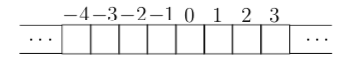
\includegraphics[scale=.8]{infinitetape.png}
    \centering
  \end{figure}

  A idéia é representar as posições $k \geq 0$ na trilha $1$ e as posições 
  menores que zero na trilha 2:

  \begin{figure}[H]
    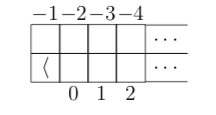
\includegraphics[scale=.8]{2tracks.png}
    \centering
  \end{figure}

  O conjunto de estados de $M'$ é $E' = E \times \{1,2\}$, que consiste de pares
  formados pelos estados de $M$ e de qual trilha (lado da fita infinita) está o
  cabeçote. O alfabeto de fita é $\Gamma' = \Gamma \cup \{\langle\}$, $i' =
  (i,1)$ e $F' = F \times \{1,2\}$. A função de transição $\delta'$ é obtida
  da seguinte forma.

  \begin{itemize}
    \item Para cada transição $\delta(e,a) = [e',b,D]$, deve-se ter: 
    \begin{itemize}
      \item $\delta'([e,1],a,c) = [[e',1],b,c,D]$, para cada $c\in \Gamma$;
      \item $\delta'([e,2],c,a) = [[e',2],c,b,D]$, para cada $c\in \Gamma$;
      \item $\delta'([e,1],\langle,a) = \delta'([e,2],\langle,a) =
        [[e',1],\langle, b,D]$.
    \end{itemize}
    \item  Para cada transição $\delta(e,a) = [e',b,E]$, deve-se ter:
    \begin{itemize}
      \item $\delta'([e,1],a,c) = [[e',1],b,c,E]$, para cada $c\in \Gamma$;
      \item $\delta'([e,2],c,a) = [[e',2],c,b,D]$, para cada $c\in \Gamma$;
      \item $\delta'([e,1],\langle,a) = \delta'([e,2],\langle,a) =
        [[e',2],\langle, b,D]$.
    \end{itemize}    
  \end{itemize}


  \section{MT com múltiplas fitas}

  Em uma MT com múltiplas fitas, cada uma das $k\geq 1$ fitas possui seu próprio
  cabeçote de leitura / escrita que podem atuar de maneira independente dos
  demais. A palavra de entrada encontra-se na fita 1 e as demais fitas são
  formadas por $\langle \sqcup^*$.

  \begin{Definition}[MT com múltiplas fitas]
    Uma MT com $k$-fitas $M = (E,\Sigma,\Gamma,\langle, \sqcup, \delta,i, F)$
    possui $E,\Sigma,\Gamma,\langle, \sqcup, i$ e $F$ como MTs padrão e a função
    de transição $\delta : E \times \Gamma^k \to E \times (\Gamma \times \{E,D,I\})^k$.
  \end{Definition}

  O uso de várias fitas pode simplificar muito o projeto de MTs. O seguinte
  exemplo ilustra esse fato.

  \begin{Example}
    A seguinte MT de duas fitas reconhece palíndromos usando a seguinte
    estratégia:
    \begin{itemize}
      \item Copia a palavra de entrada para a fita 2.
      \item Volta o cabeçote da fita 1 para o início enquanto o da fita 2 fica
        no último símbolo da palavra de entrada.
      \item Inicia a comparação, símbolo a símbolo, dos símbolos sobre o
        cabeçote de cada fita.
      \end{itemize}
      \begin{figure}[H]
       \begin{tikzpicture}[node distance=3.5cm]
        \node[state, initial](s0){$A$} ;
        \node[state, right of=s0](s1){$B$};
        \node[state, right of=s1](s2){$C$};
        \node[state, accepting, below of=s2](s3){$D$};
        \draw (s0) edge[loop above]node{$\begin{array}{c}1/1\:D;\sqcup/1\:D\\0/0\:D;\sqcup/0\:D\\\end{array}$}(s0)
              (s0) edge[above]node{$\sqcup/\sqcup\:E; \sqcup/\sqcup\:E$}(s1)
              (s1) edge[loop above]node{$\begin{array}{c}0/0\:E;*/*\:I\\1/1\:E;*/*\:I\end{array}$}(s1)
              (s1) edge[above]node{$\langle / \langle\: D; */*\:I$} (s2)
              (s2) edge[loop above]node{$\begin{array}{c}0/0\:D;0/0\:E\\1/1\:D;1/1\:E\end{array}$}(s2)
              (s2) edge[right]node{$\sqcup/\sqcup\:E;\langle / \langle\:D$}(s3);
        \end{tikzpicture}       
        \centering
      \end{figure}
  \end{Example}

  Para mostrar a equivalência de MTs com várias fitas e a MT padrão, mostremos
  como uma MT de $2$-fitas pode ser simulada por uma MT de $4$ trilhas.
  A idéia é usar a trilha $1$ para armazenar o conteúdo da fita $1$ e a trilha 2
  armazena um símbolo $X \not\in \Gamma$ que indica a posição atual do cabeçote
  na fita $1$. O mesmo raciocínio aplica-se a fita 2 e trilhas 3 e 4. Após a
  escrita da posição inicial dos cabeçotes das fitas 1 e 2 nas trilhas 2 e 4,
  escrever $\langle$ no início da trilha 3. Transições da nova MT simulam
  as transições realizadas pela MT de duas fitas e atualizam as trilhas 2 e 4
  para refletir a movimentação do cabeçote.

  \section{MT não determinísticas}

  Um MT não determinística é uma MT que admite mais de uma transição partindo
  de um certo estado sobre um certo símbolo. Em uma MT não determinística,
  a aceitação de uma palavra é determinada pela existência de uma computação
  que pára em estado final.

 \begin{Definition}[MT não determinística]
    Uma MT não determinística $M = (E,\Sigma,\Gamma,\langle, \sqcup, \delta,i, F)$
    possui $E,\Sigma,\Gamma,\langle, \sqcup, i$ e $F$ como MTs padrão e a função
    de transição $\delta : E \times \Gamma \to \mathcal{P}(E \times (\Gamma \times \{E,D,I\})$.
  \end{Definition}

  Evidentemente, o uso de não-determinismo simplifica muito o projeto de MTs.
  A seguir, ilustramos isso usando um exemplo.

  \begin{Example}
    Considere uma MT não determinística de duas fitas para a linguagem
    $\{xx\,|\,x \in \{0,1\}^*\}$:
    \begin{figure}[H]
       \begin{tikzpicture}[node distance=3.5cm]
        \node[state, initial](s0){$A$} ;
        \node[state, right of=s0](s1){$B$};
        \node[state, right of=s1](s2){$C$};
        \node[state, accepting, below of=s2](s3){$D$};
        \draw (s0) edge[loop above]node{$\begin{array}{c}1/1\:D;\sqcup/1\:D\\0/0\:D;\sqcup/0\:D\\\end{array}$}(s0)
              (s0) edge[above]node{$\begin{array}{c}1/1\:I;\sqcup/\sqcup\:E\\0/0\:I;\sqcup/\sqcup\:E\\\end{array}$}(s1)
              (s1) edge[loop above]node{$\begin{array}{c}0/0\:I;*/*\:E\\1/1\:I;*/*\:E\end{array}$}(s1)
              (s1) edge[above]node{$\langle / \langle\: D;\langle / \langle\: D$} (s2)
              (s2) edge[loop above]node{$\begin{array}{c}0/0\:D;0/0\:D\\1/1\:D;1/1\:D\end{array}$}(s2)
              (s2) edge[right]node{$*/*\:D;\sqcup / \sqcup\:D$}(s3);
        \end{tikzpicture}       
        \centering
      \end{figure}    
  \end{Example}

  Pode-se simular uma MT não determinística usando uma MT determinística de 3
  fitas. A idéia é simular, sistematicamente, todas as computações de tamanho
  $n$ antes de tentar uma possuindo $n + 1$ passos. A execução da MT de 3 fitas
  procede de acordo com o seguinte algoritmo:
  \begin{enumerate}
    \item Inicialize a fita 3 com a palavra 1.
    \item repita 
    \begin{enumerate}
      \item copie a palavra de entrada da fita 1 para a fita 2.
      \item Simule M na fita 2 de acordo com a palavra na fita 3.
      \item se M parar em estado final, aceite.
      \item apague a fita 2.
      \item gere a próxima palavra para a fita 3.
    \end{enumerate}
  \end{enumerate}
  É importante notar que as palavras na fita 3 representam possíveis transições
  não deterministas de $M$. Se $n$ é o número máximo de transições não
  determinísticas em $M$, pode numerar as transições da MT usando palavras
  formadas por símbolos do conjunto $\{1..n\}$. Cada transição recebe um número
  e palavras sobre esse alfabeto representam computações em M seguindo as
  transições correspondentes a estes números.

  Dessa forma, temos a equivalência entre MTs não determinísticas e MTs padrão.

  \section{Exercícios}

  \begin{enumerate}
     \item Construa uma MT não determinística de duas fitas que reconheça a
       linguagem $\{w\,|\,\eta_0(w) = \eta_1(w)\}$.
     \item Construa uma MT de duas fitas que reconheça $\{wcw\,|\,w \in
       \{0,1\}^*\}$.
  \end{enumerate}
\end{document}
